\documentclass{scrreprt}
\usepackage{listings}
\usepackage{underscore}
\usepackage[bookmarks=true]{hyperref}
\hypersetup{
    bookmarks=false,    % show bookmarks bar?
    pdftitle={User Manual},    % title
    pdfauthor={Yiannis Lazarides},                     % author
    pdfsubject={TeX and LaTeX},                        % subject of the document
    pdfkeywords={TeX, LaTeX, graphics, images}, % list of keywords
    colorlinks=true,       % false: boxed links; true: colored links
    linkcolor=blue,       % color of internal links
    citecolor=black,       % color of links to bibliography
    filecolor=black,        % color of file links
    urlcolor=purple,        % color of external links
    linktoc=page            % only page is linked
}%
\title{\flushright
%\rule{16cm}{5pt}\vskip1cm
\Huge{User Manual}\\
\vspace{2cm}
for\\
\vspace{2cm}
Potku\\
\vspace{2cm}
\LARGE{Updated version 2013.07.23\\}
\vspace{2cm}
\LARGE{Created version 2013.07.19\\}
%\LARGE{Version \myversion approved\\}
\vspace{2cm}
Prepared by Timo Konu\\
\vfill
%\rule{16cm}{5pt}
}
\date{}
\usepackage{hyperref}
\usepackage{graphicx}
\usepackage{float}

\begin{document}
\maketitle
\tableofcontents
\chapter{Introduction}
\section{Purpose}
Potku is a graphical user interface for analysis and visualization of a ToF-ERD telescope's measurement data. For physics calculations Potku uses external analysis components.

The Potku software can draw the data points received from the telescope into a histogram, allow the user to select chemical elements from the histogram, and use the selected elements to produce elemental losses histograms, energy spectrum histograms and depth profile histograms.

The software was developed with Python 3.3, PyQt and MatplotLib. External analysis components are written in C.

\section{Installation}
The installation instructions can be found in the downloaded package as installing_instructions.txt file.
\chapter{Individual sections}
%%%%%%%%%%%%%
%%%%%%%%%%%%% MAIN WINDOW
%%%%%%%%%%%%%
\section{Main Window}\label{mainwindow}
\begin{figure}[H]
\centering
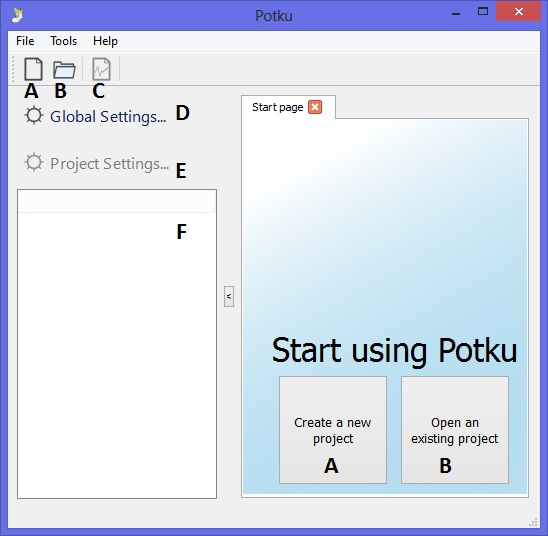
\includegraphics[height=90mm]{mainwindow}
\caption{The main window of Potku}
\label{fig-mainwindow}
\end{figure}
Explanation for the objects in the main window in the figure \ref{fig-mainwindow}:

\begin{tabular}{ll}
A & Create a new project. Section \ref{projectdialog}.\\
B & Open a project.\\
C & Load a measurement into a project.\\
D & Change global settings of Potku. Section \ref{globalsettings}.\\
E & Change project specific settings. Section \ref{projectsettings}.\\
F & A list of measurements in a project.\\
\end{tabular}

%%%%%%%%%%%%%
%%%%%%%%%%%%% MENUBAR
%%%%%%%%%%%%%
\section{Menubar}\label{menubar}
\begin{figure}[H]
\centering
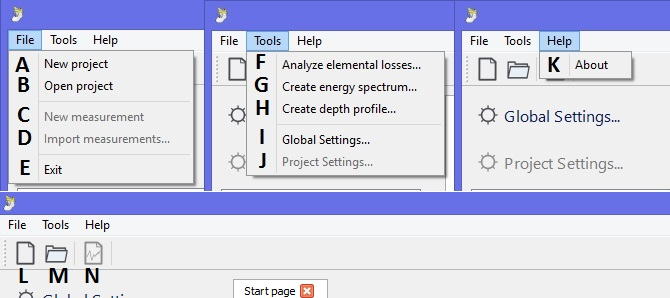
\includegraphics[width=140mm]{menubar}
\caption{The menubar of main window of Potku}
\label{fig-menubar}
\end{figure}
Explanation for the objects of menubar in the figure \ref{fig-menubar}:

\begin{tabular}{ll}
A & Create a new project. Section \ref{projectdialog}.\\
B & Open a project.\\
C & Load a measurement into a project.\\
D & Import measurements directly from ToF-Erda measuring unit. Section \ref{importdialog}.\\
E & Exit Potku.\\
F & Open a dialog for elemental losses analysis for an active measurement. Section \ref{measurement-dialogelemloss}.\\
G & Open a dialog for energy spectrum analysis for an active measurement. Section \ref{measurement-dialogenergy}.\\
H & Open a dialog for depth profile analysis for an active measurement. Section \ref{measurement-dialogdepth}.\\
I & Change global settings of Potku. Section \ref{globalsettings}.\\
J & Change project specific settings. Section \ref{projectsettings}.\\
K & Open the about dialog of Potku.\\
L & Create a new project. Section \ref{projectdialog}.\\
M & Open a project.\\
N & Load a measurement into a project.\\
\end{tabular}

%%%%%%%%%%%%%
%%%%%%%%%%%%% NEW PROJECT DIALOG
%%%%%%%%%%%%%
\section{New Project Dialog}\label{projectdialog}
\begin{figure}[H]
\centering
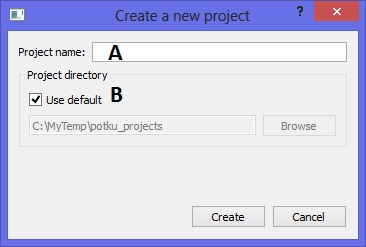
\includegraphics[scale=1]{projectdialog}
\caption{The dialog for creating a new project.}
\label{fig-projectdialog}
\end{figure}
Explanation for the objects in the figure \ref{fig-projectdialog}:

\begin{tabular}{ll}
A & A name for the project.\\
B & A location where the project will be saved to.\\
\end{tabular}

%%%%%%%%%%%%%
%%%%%%%%%%%%% GLOBAL SETTINGS
%%%%%%%%%%%%%
\section{Global Settings}\label{globalsettings}
\begin{figure}[H]
\centering
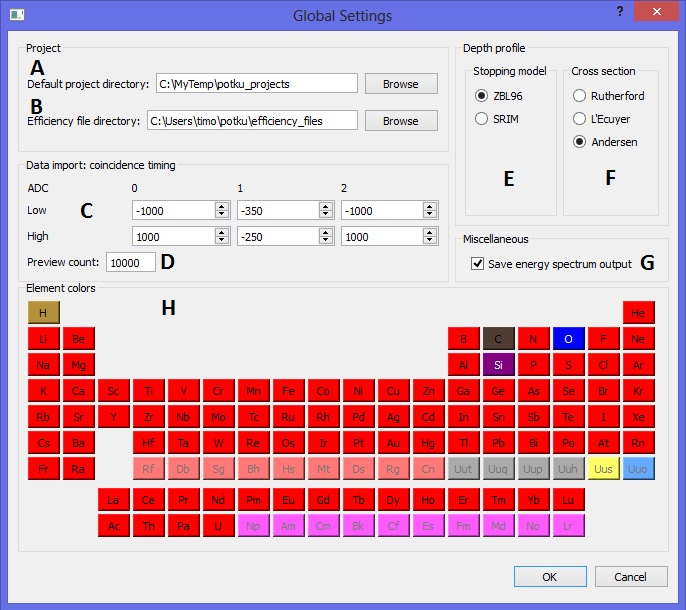
\includegraphics[width=140mm]{globalsettings}
\caption{The global settings dialog of Potku}
\label{fig-globalsettings}
\end{figure}
Explanation for the objects in the global settings dialog in the figure \ref{fig-globalsettings}:

\begin{tabular}{ll}
A & Default directory where all new projects will be saved to.\\
B & Directory where energy spectrum and depth profile check for efficiency files.\\
C & Coincidency timing windows for different ADC triggers used when importing \\&measurement data of ToF-Erda measuring unit. Section \ref{importdialog}.\\
D & Maximum number of coincidences when previewing import timings. Section \ref{importprevdialog}.\\
E & Stopping model options for depth profile.\\
F & Cross section options for depth profile.\\
G & Option to save tof_in (external program) output from energy spectrum.\\
H & Default colors for each element.\\
\end{tabular}

%%%%%%%%%%%%%
%%%%%%%%%%%%% PROJECT SETTINGS
%%%%%%%%%%%%%
\section{Project Settings}\label{projectsettings}
\begin{figure}[H]
\centering
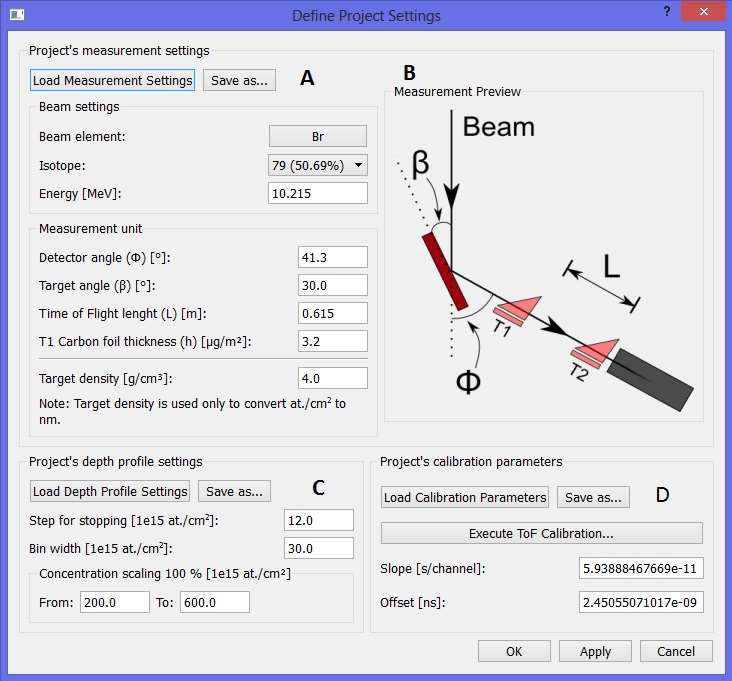
\includegraphics[width=140mm]{projectsettings}
\caption{The project settings dialog of Potku}
\label{fig-projectsettings}
\end{figure}
Explanation for the objects in the project settings dialog in the figure \ref{fig-projectsettings}:

\begin{tabular}{ll}
A & Settings specified for measurement unit.\\
B & A figure explaining all measurement unit settings.\\
C & Settings used to make depth profile.\\
D & Calibration settings values. Section \ref{measurement-tofe-calib-curve}.\\
\end{tabular}

%%%%%%%%%%%%%
%%%%%%%%%%%%% IMPORT DIALOG
%%%%%%%%%%%%%
\section{Import Dialog}\label{importdialog}
\begin{figure}[H]
\centering
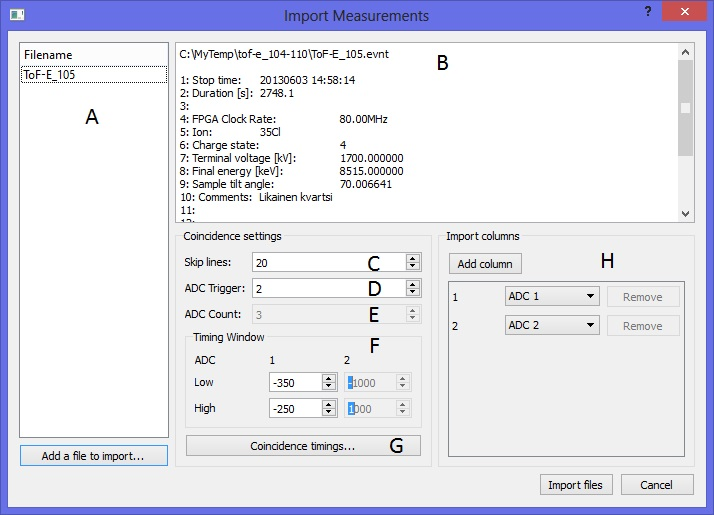
\includegraphics[width=140mm]{importdialog}
\caption{The import dialog of Potku}
\label{fig-importdialog}
\end{figure}
Explanation for the objects in the import dialog in the figure \ref{fig-importdialog}:

\begin{tabular}{ll}
A & A list of measurement unit's data files to be imported into open project.\\
B & A preview of the selected measurement file.\\
C & A value determining how many lines from the beginning of the file(s) is skipped when importing.\\
D & An ADC trigger channel.\\
E & Total amount of ADC channels in file(s).\\
F & Time difference values for different ADC channels to find coincidences.\\
G & Opens preview of selected file with time difference values. Section \ref{importprevdialog}.\\
H & Columns that are added to the imported file(s).\\
\end{tabular}

%%%%%%%%%%%%%
%%%%%%%%%%%%% IMPORT DIALOG PREVIEW
%%%%%%%%%%%%%
\section{Coincidence Timing Preview}\label{importprevdialog}
\begin{figure}[H]
\centering
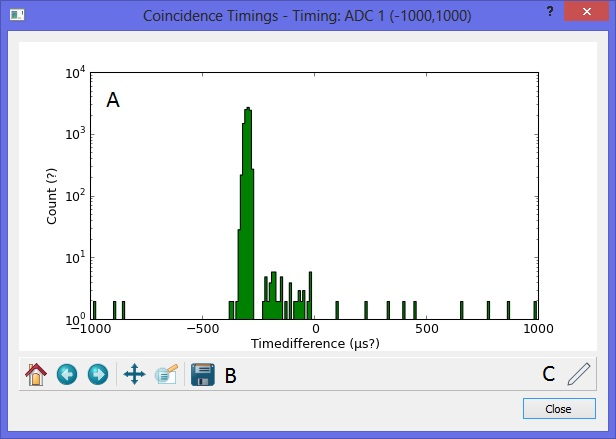
\includegraphics[width=140mm]{importprevdialog}
\caption{The import dialog of Potku}
\label{fig-importprevdialog}
\end{figure}
Explanation for the objects in the coincidence timing preview dialog in the figure \ref{fig-importprevdialog}:

\begin{tabular}{ll}
A & A graph which shows found coincidences between the selected timing window.\\
B & A toolset provided to pan, zoom and save the graph.\\
C & A tool for manually selecting a good coincidence timing window.\\
\end{tabular}

%%%%%%%%%%%%%
%%%%%%%%%%%%% MEASUREMENT TAB
%%%%%%%%%%%%%
\section{Measurement Tabs}\label{measurementtab}
\begin{figure}[H]
\centering
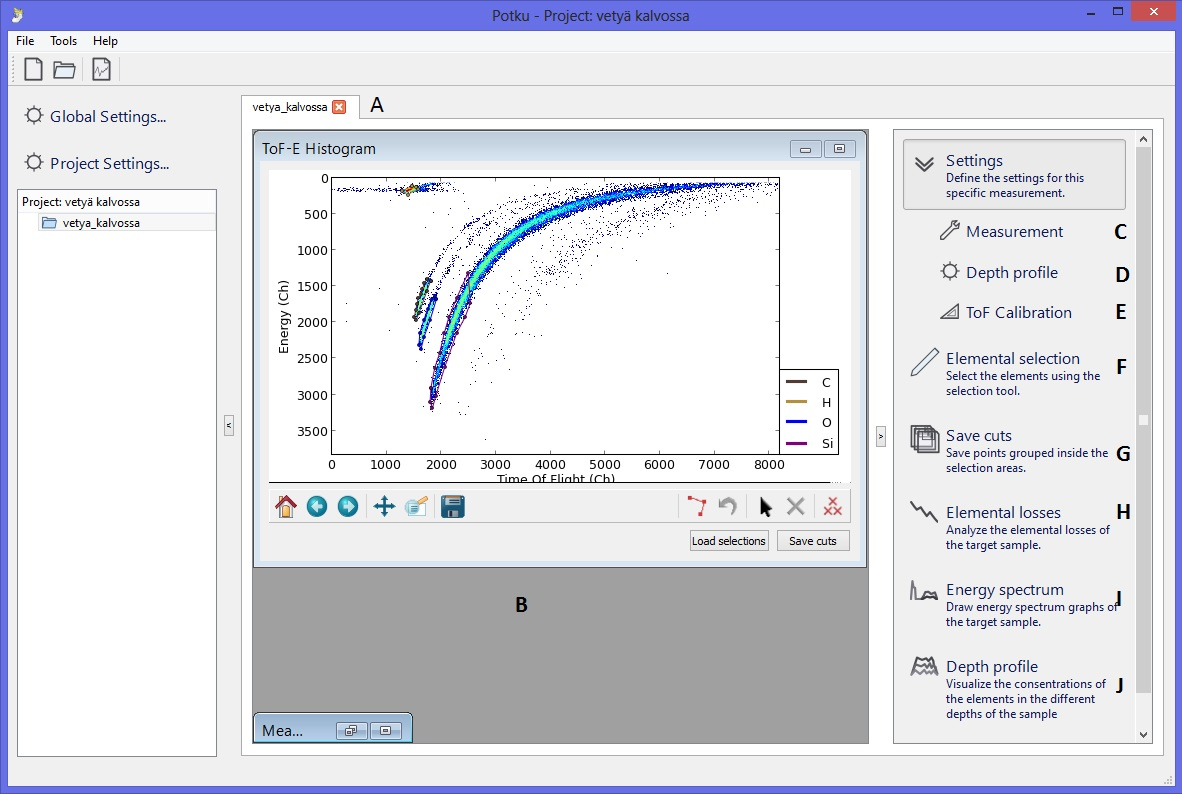
\includegraphics[width=140mm]{mainwindow-measurementtab}
\caption{The measurement tabs of Potku}
\label{fig-measurementtab}
\end{figure}
Explanation for the objects in the measurement tabs in the figure \ref{fig-measurementtab}:

\begin{tabular}{ll}
A & All open measurements in the tabs.\\
B & The workspace of an active measurement. Section \ref{measurementtab-content}\\
C & Measurement unit settings for active measurement. See \ref{measurement-measurementsettings}\\
D & Depth profile settings for active measurement. See \ref{measurement-depthsettings}\\
E & ToF-E Calibration settings for active measurement. See \ref{measurement-calibsettings}\\
F & Enable element selection tool in ToF-E histogram. See \ref{measurementtab-tofe}\\
G & Save element selection data in ToF-E histogram. See \ref{measurementtab-tofe}\\
H & Open the elemental losses dialog. See \ref{measurement-dialogelemloss}\\
I & Open the energy spectrum dialog. See \ref{measurement-dialogenergy}\\
J & Open the depth profile dialog. See \ref{measurement-dialogdepth}\\
\end{tabular}

%%%%%%%%%%%%%
%%%%%%%%%%%%% MEASUREMENT - MEASUREMENT SETTINGS
%%%%%%%%%%%%%
\section{Measurement's Measurement Settings}\label{measurement-measurementsettings}
\begin{figure}[H]
\centering
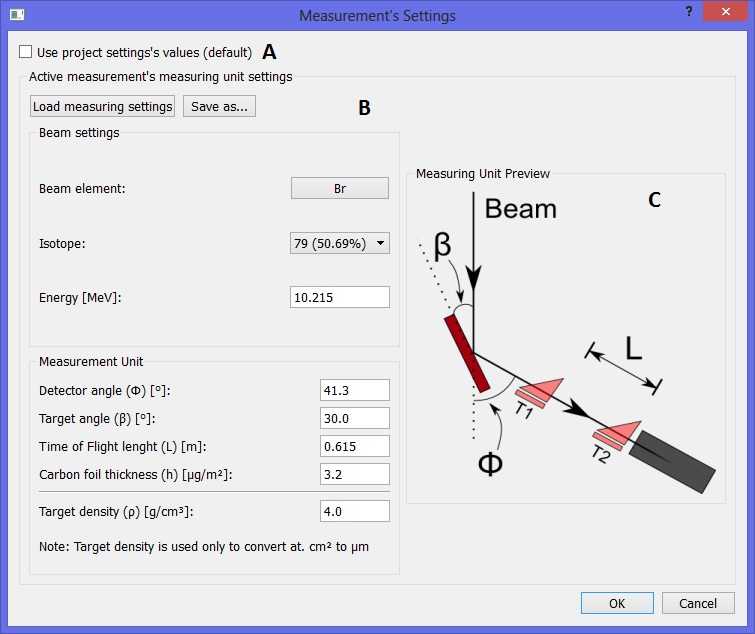
\includegraphics[width=140mm]{measurement-measurementsettings}
\caption{The measurement's measurement settings dialog of Potku}
\label{fig-measurementsettings}
\end{figure}
Explanation for the objects in the measurement's measurement settings in the figure \ref{fig-measurementsettings}:

\begin{tabular}{ll}
A & Toggle whether measurement uses project's settings or its own.\\
B & Settings specified for measurement unit.\\
C & A figure explaining all measurement unit settings.\\
\end{tabular}

%%%%%%%%%%%%%
%%%%%%%%%%%%% MEASUREMENT - DEPTH PROFILE SETTINGS
%%%%%%%%%%%%%
\section{Measurement's Depth Profile Settings}\label{measurement-depthsettings}
\begin{figure}[H]
\centering
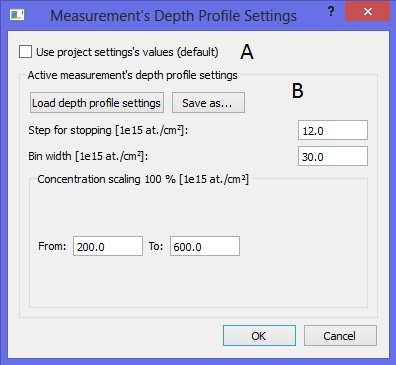
\includegraphics[scale=1]{measurement-depthsettings}
\caption{The measurement's depth profile settings dialog of Potku}
\label{fig-depthsettings}
\end{figure}
Explanation for the objects in the measurement's depth profile settings in the figure \ref{fig-depthsettings}:

\begin{tabular}{ll}
A & Toggle whether measurement uses project's settings or its own.\\
B & Settings used to make depth profile.\\
\end{tabular}

%%%%%%%%%%%%%
%%%%%%%%%%%%% MEASUREMENT - CALIBRATION SETTINGS
%%%%%%%%%%%%%
\section{Measurement's ToF-E Calibration Settings}\label{measurement-calibsettings}
\begin{figure}[H]
\centering
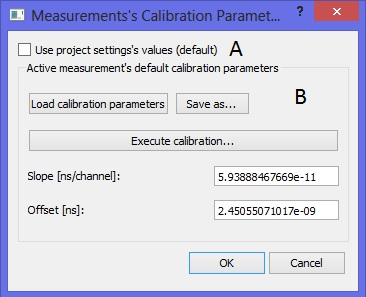
\includegraphics[scale=1]{measurement-calibsettings}
\caption{The measurement's ToF-E calibration settings dialog of Potku}
\label{fig-calibsettings}
\end{figure}
Explanation for the objects in the measurement's ToF-E calibration settings in the figure \ref{fig-calibsettings}:

\begin{tabular}{ll}
A & Toggle whether measurement uses project's settings or its own.\\
B & Calibration settings values. Section \ref{measurement-tofe-calib-curve}.\\
\end{tabular}

%%%%%%%%%%%%%
%%%%%%%%%%%%% MEASUREMENT TAB - ELEMENTAL LOSSES DIALOG
%%%%%%%%%%%%%
\section{Measurement's Elemental Losses Dialog}\label{measurement-dialogelemloss}
\begin{figure}[H]
\centering
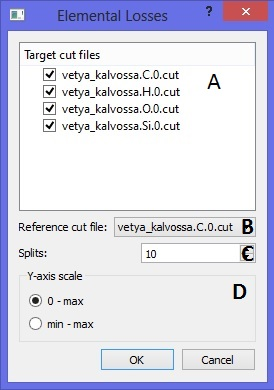
\includegraphics[scale=1]{measurement-dialogelemloss}
\caption{The measurement's elemental losses dialog of Potku}
\label{fig-dialogelemloss}
\end{figure}
Explanation for the objects in the measurement's elemental losses dialog in the figure \ref{fig-dialogelemloss}:

\begin{tabular}{ll}
A & A list of saved cut files in the measurement.\\
B & A saved cut file that is used as reference for losses.\\
C & A setting to define to how many splits cut files are split.\\
D & Different options for Y axis scaling.\\
\end{tabular}

%%%%%%%%%%%%%
%%%%%%%%%%%%% MEASUREMENT TAB - ENERGY SPECTRUM DIALOG
%%%%%%%%%%%%%
\section{Measurement's Energy Spectrum Dialog}\label{measurement-dialogenergy}
\begin{figure}[H]
\centering
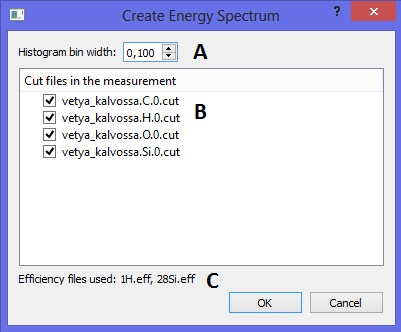
\includegraphics[scale=1]{measurement-dialogenergy}
\caption{The measurement's energy spectrum dialog of Potku}
\label{fig-dialogenergy}
\end{figure}
Explanation for the objects in the measurement's elemental losses dialog in the figure \ref{fig-dialogenergy}:

\begin{tabular}{ll}
A & Histogram bin width.\\
B & A list of saved cut files in the measurement.\\
C & A list of efficiency files found for the cut files.\\
\end{tabular}

%%%%%%%%%%%%%
%%%%%%%%%%%%% MEASUREMENT TAB - DEPTH PROFILE DIALOG
%%%%%%%%%%%%%
\section{Measurement's Depth Profile Dialog}\label{measurement-dialogdepth}
\begin{figure}[H]
\centering
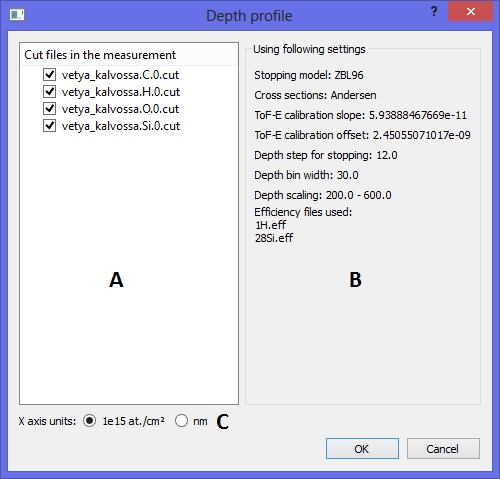
\includegraphics[scale=1]{measurement-dialogdepth}
\caption{The measurement's depth profile dialog of Potku}
\label{fig-dialogdepth}
\end{figure}
Explanation for the objects in the measurement's depth profile dialog in the figure \ref{fig-dialogdepth}:

\begin{tabular}{ll}
A & A list of saved cut files in the measurement.\\
B & Combination of all settings that are used to create depth profile\\
C & X axis options for depth profile.\\
\end{tabular}

%%%%%%%%%%%%%
%%%%%%%%%%%%% MEASUREMENT TAB
%%%%%%%%%%%%%
\section{Measurement's Workspace}\label{measurementtab-content}
Active measurement's workspace, see figure \ref{fig-measurementtab}, has subwindows for Tof-E histogram (Section \ref{measurementtab-tofe}),
elemental losses (Section \ref{measurementtab-elemloss}), energy spectrum (Section \ref{measurementtab-energy}), 
depth profile (Section \ref{measurementtab-depth}) and measurement log (Section \ref{measurementtab-log}).

%%%%%%%%%%%%%
%%%%%%%%%%%%% MEASUREMENT TAB - TOF-E HISTOGRAM
%%%%%%%%%%%%%
\section{ToF-E Histogram}\label{measurementtab-tofe}
\begin{figure}[H]
\centering
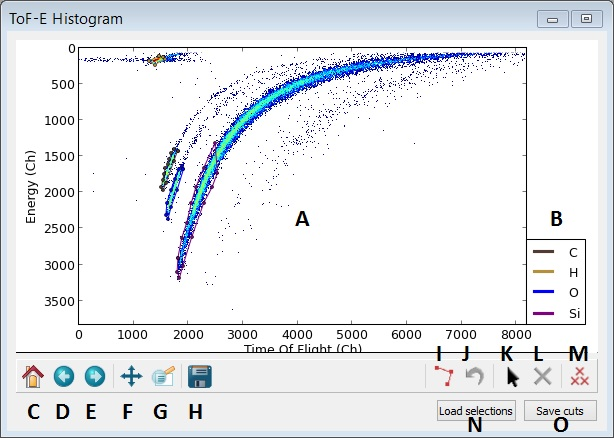
\includegraphics[width=140mm]{measurement-tofe}
\caption{The ToF-E histogram of an active measurement.}
\label{fig-tofe}
\end{figure}
Explanation for the objects in the figure \ref{fig-tofe}:

\begin{tabular}{ll}
A & A histogram graph for time-of-Flight and energy.\\
B & A legend box where all selected elements are shown.\\
C & Reset graph to its original position.\\
D & Go to previous view if the user has panned or zoomed the graph.\\
E & Go to next view if the user has panned or zoomed the graph.\\
F & Pan the graph.\\
G & Zoom in or out the graph.\\
H & Save the graph as an image file.\\
I & An element selection tool which is used to select elements from ToF-E histogram.\\
J & Undo a node in an open element selection.\\
K & A tool to highlight an element selection.\\
L & Delete a highlighted element selecetion.\\
M & Delete all element selsections.\\
N & Load a selection file containing selections.\\
O & Save the element selections to cut files.\\
\end{tabular}

%%%%%%%%%%%%%
%%%%%%%%%%%%% MEASUREMENT TAB - ELEMENTAL LOSSES
%%%%%%%%%%%%%
\section{Elemental Losses}\label{measurementtab-elemloss}
\begin{figure}[H]
\centering
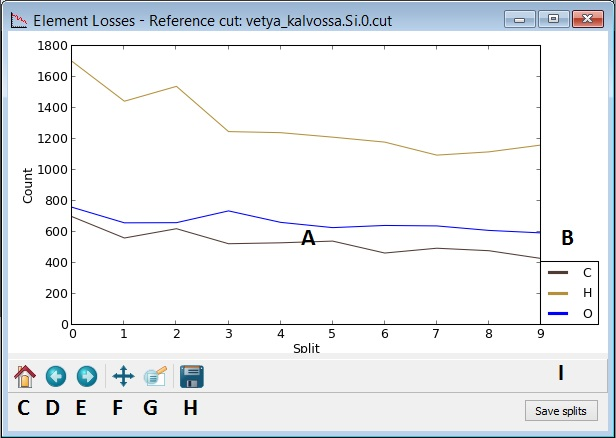
\includegraphics[width=140mm]{measurement-elemloss}
\caption{The histogram of elemental losses of an active measurement.}
\label{fig-elemloss}
\end{figure}
Explanation for the objects in the figure \ref{fig-elemloss}:

\begin{tabular}{ll}
A & A histogram graph for splits and counts within splits.\\
B & A legend box where all selected elements are shown.\\
C & Reset graph to its original position.\\
D & Go to previous view if the user has panned or zoomed the graph.\\
E & Go to next view if the user has panned or zoomed the graph.\\
F & Pan the graph.\\
G & Zoom in or out the graph.\\
H & Save the graph as an image file.\\
I & Save splitted cut files into new cut files.\\
\end{tabular}

%%%%%%%%%%%%%
%%%%%%%%%%%%% MEASUREMENT TAB - ENERGY SPECTRUM
%%%%%%%%%%%%%
\section{Energy Spectrum}\label{measurementtab-energy}
\begin{figure}[H]
\centering
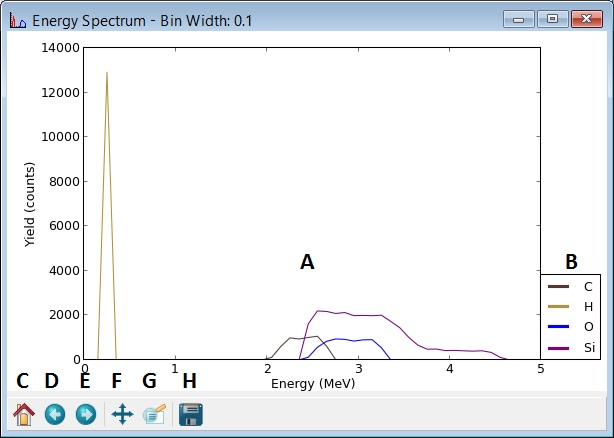
\includegraphics[width=140mm]{measurement-energy}
\caption{The histogram of energy spectrum of an active measurement.}
\label{fig-energy}
\end{figure}
Explanation for the objects in the figure \ref{fig-energy}:

\begin{tabular}{ll}
A & A histogram graph for energy and yield.\\
B & A legend box where all selected elements are shown.\\
C & Reset graph to its original position.\\
D & Go to previous view if the user has panned or zoomed the graph.\\
E & Go to next view if the user has panned or zoomed the graph.\\
F & Pan the graph.\\
G & Zoom in or out the graph.\\
H & Save the graph as an image file.\\
\end{tabular}

%%%%%%%%%%%%%
%%%%%%%%%%%%% MEASUREMENT TAB - DEPTH PROFILE
%%%%%%%%%%%%%
\section{Depth Profile}\label{measurementtab-depth}
\begin{figure}[H]
\centering
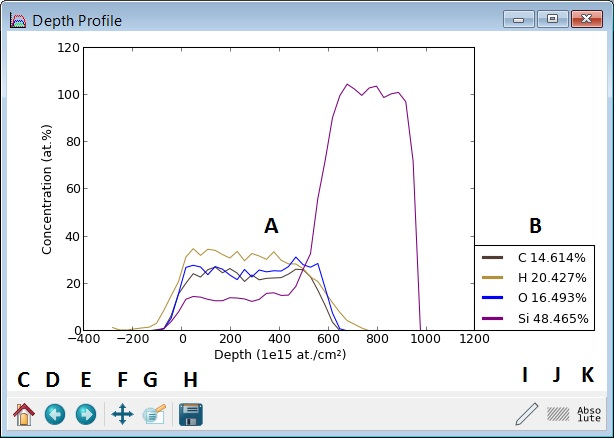
\includegraphics[width=140mm]{measurement-depth}
\caption{The histogram of depth profile of an active measurement.}
\label{fig-depth}
\end{figure}
Explanation for the objects in the figure \ref{fig-depth}:

\begin{tabular}{ll}
A & A histogram graph for depth and concentration.\\
B & A legend box where all selected elements and their percentages are shown.\\
C & Reset graph to its original position.\\
D & Go to previous view if the user has panned or zoomed the graph.\\
E & Go to next view if the user has panned or zoomed the graph.\\
F & Pan the graph.\\
G & Zoom in or out the graph.\\
H & Save the graph as an image file.\\
I & Set bondaries from the element percentages are calculated from.\\
J & Set area which is affect by the button K.\\
K & Toggle between absolute and relative plotting of the graph.\\
\end{tabular}

%%%%%%%%%%%%%
%%%%%%%%%%%%% MEASUREMENT TAB - LOG
%%%%%%%%%%%%%
\section{Measurement Log}\label{measurementtab-log}
\begin{figure}[H]
\centering
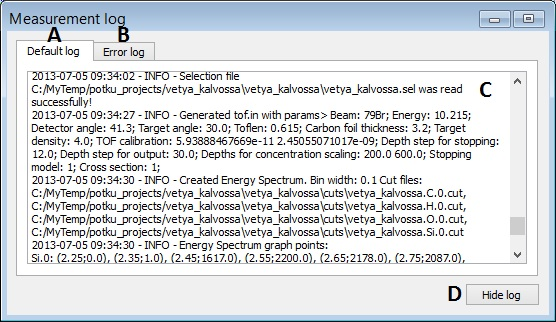
\includegraphics[width=140mm]{measurement-log}
\caption{The log window of an active measurement.}
\label{fig-log}
\end{figure}
Explanation for the objects in the figure \ref{fig-log}:

\begin{tabular}{ll}
A & A log tab for all messages regarding the measurement.\\
B & A log tab for only error events.\\
C & Log content.\\
D & Minimize the log window.\\
\end{tabular}

%%%%%%%%%%%%%
%%%%%%%%%%%%% TOF-E HISTOGRAM - GRAPH SETTINGS
%%%%%%%%%%%%%
\section{ToF-E Histogram Graph Settings}\label{measurement-tofe-settings}
\begin{figure}[H]
\centering
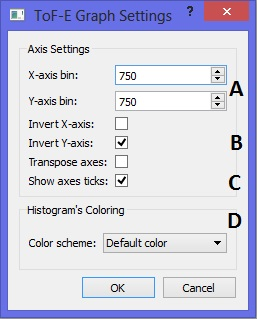
\includegraphics[scale=1]{measurement-tofe-settings}
\caption{The graph settings window of ToF-E Histogram.}
\label{fig-tofe-settings}
\end{figure}
Explanation for the objects in the figure \ref{fig-tofe-settings}:

\begin{tabular}{ll}
A & Bin width for X and Y axes.\\
B & Options to invert and transpose axes.\\
C & Show axes units and ticks.\\
D & Color scheme used for the graph.\\
\end{tabular}

%%%%%%%%%%%%%
%%%%%%%%%%%%% TOF-E HISTOGRAM - ELEMENT SELECTION
%%%%%%%%%%%%%
\section{ToF-E Histogram Element Selection}\label{measurement-tofe-element}
\begin{figure}[H]
\centering
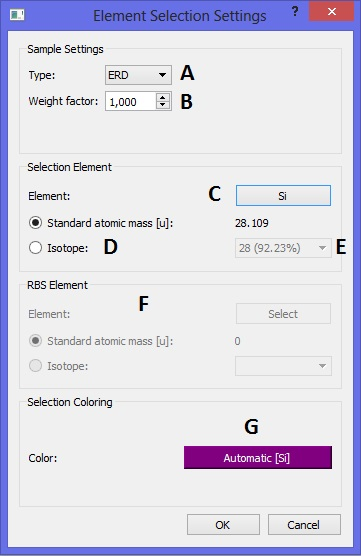
\includegraphics[scale=1]{measurement-tofe-element}
\caption{The element selection.}
\label{fig-tofe-element}
\end{figure}
Explanation for the objects in the figure \ref{fig-tofe-element}:

\begin{tabular}{ll}
A & A selection for element type (ERD/RBS).\\
B & A weight factor for the element.\\
C & A button to choose selection element.\\
D & An option to choose between standard and specific isotope of the element.\\
E & A selection for specific isotope.\\
F & Settings for RBS selection.\\
G & A color selector for the element selection.\\
\end{tabular}

%%%%%%%%%%%%%
%%%%%%%%%%%%% TOF-E CALIBRATION - CURVE FITTING
%%%%%%%%%%%%%
\section{ToF-E Calibration Fitting}\label{measurement-tofe-calib-curve}
\begin{figure}[H]
\centering
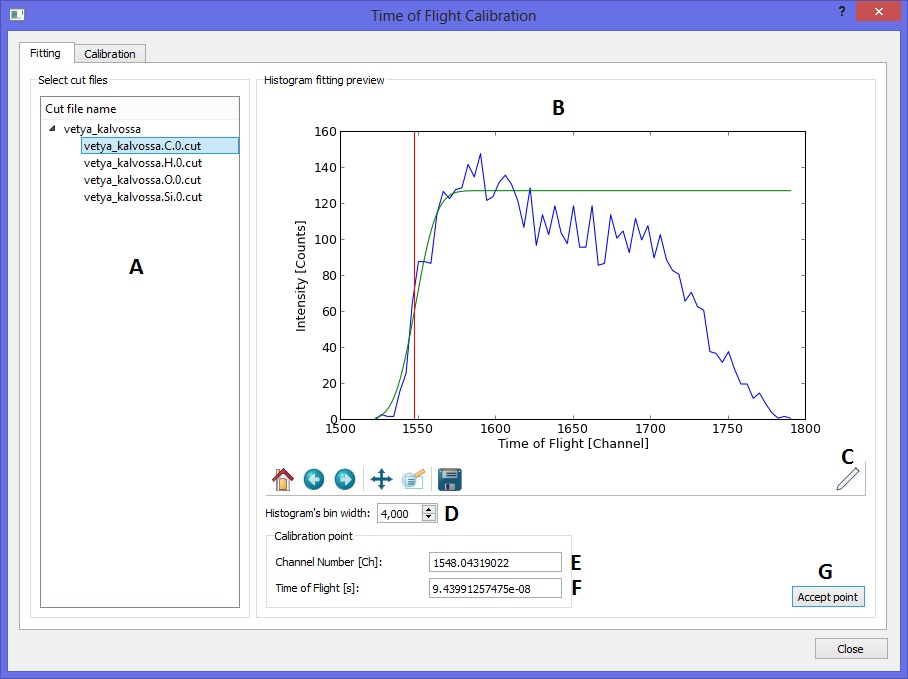
\includegraphics[width=140mm]{measurement-tofe-calib-curve}
\caption{The calibration window for fitting.}
\label{fig-tofe-calib-curve}
\end{figure}
Explanation for the objects in the figure \ref{fig-tofe-calib-curve}:

\begin{tabular}{ll}
A & A list of cut files of measurements in the project.\\
B & A fitting graph and front edge estimation.\\
C & A tool to manually select front edge if estimation is incorrect.\\
D & An option to change bin width size.\\
E & An estimated front edge channel.\\
F & A theoretical time-of-flight for the element of a cut file.\\
G & Accept front edge estimation to calibration. Section \ref{measurement-tofe-calib-linear}.\\
\end{tabular}

%%%%%%%%%%%%%
%%%%%%%%%%%%% TOF-E CALIBRATION - LINEAR FITTING
%%%%%%%%%%%%%
\section{ToF-E Calibration}\label{measurement-tofe-calib-linear}
\begin{figure}[H]
\centering
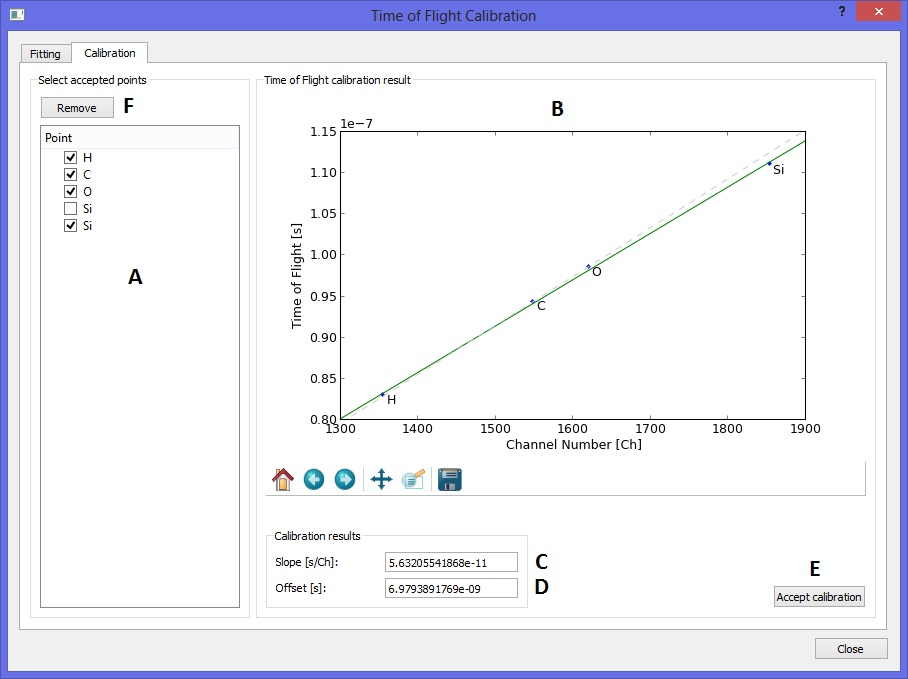
\includegraphics[width=140mm]{measurement-tofe-calib-linear}
\caption{The calibration window.}
\label{fig-tofe-calib-linear}
\end{figure}
Explanation for the objects in the figure \ref{fig-tofe-calib-linear}:

\begin{tabular}{ll}
A & A list of accepted front edges from fitting. Section \ref{fig-tofe-calib-curve}.\\
B & A calibration graph for and comparison to previous ToF-E Calibration.\\
C & The slope of the calibration.\\
D & The offset of the calibration.\\
E & Accept current calibration as ToF-E calibration.\\
F & Remove selected curve fitting points from the list.\\
\end{tabular}


\chapter{Using Potku}
%%%%%%%%%%%%%
%%%%%%%%%%%%% HOW TO - PROJECT
%%%%%%%%%%%%%
\section{How To Make A Project}\label{howto-project}
To create a new project user selects create a new project from main window after starting Potku or new project from menubar. 
Both of these will open a dialog, shown in Section \ref{projectdialog}, where user has to set the name and location of the project.
The project requires a name which has to be a valid format for a folder name, since all measurements will be saved there.
The project is saved to user's documents folder by default but this can be changed by unchecking ''Use default'' and browsing to a new location.
The default folder can be changed in global settings, shown in Section \ref{globalsettings}.

%%%%%%%%%%%%%
%%%%%%%%%%%%% HOW TO - ADD MEASUREMENT (LOAD/IMPORT)
%%%%%%%%%%%%%
\section{How To Add Measurement To A Project}\label{howto-measurement}
Adding a new measurement to a project after creating, Section \ref{howto-project}, or opening a project will happen through loading or importing measurement, which can be found in menubar Section \ref{menubar}.
Loading a measurement is straightforward process where user has to browse to measurement's .asc file location and load it.
Importing a measurement, Section \ref{howto-measurement-import}, process imports raw measurement information from a ToF-E measuring unit into an .asc file used by Potku.

%%%%%%%%%%%%%
%%%%%%%%%%%%% HOW TO - IMPORT MEASUREMENT
%%%%%%%%%%%%%
\subsection{How To Import Measurement To A Project}\label{howto-measurement-import}
After saving a raw measurement data file(s) from a ToF-E measuring unit; these can imported using import dialog, Section \ref{importdialog}.
After adding the files to the list of measurements-to-be-imported. Potku will automatically seek the first line of the actual data and different ADC triggers found in the file.
Suitable coincidence timing for ADC channel(s) can be selected via the coincidence timing preview window, Section \ref{importprevdialog}.
User can select the suitable range, which is around the highest peak where the most coincidences happen, with the manual selection tool.
User can then select from predefined options what columns will be imported. By default the default ADC channels will be included.

%%%%%%%%%%%%%
%%%%%%%%%%%%% HOW TO - SETTINGS
%%%%%%%%%%%%%
\section{How To Set Measurement Settings}\label{howto-settings}
Changing the measurement units parameters for project happens in Project Settings window. You can find this button in main window of Potku, Section \ref{mainwindow}.
Content of the window is explained in Section \ref{projectsettings}.
If user has a measurement open and wants to change settings for this specific measurement, the button for this can be found under Settings as Measurement shown in Section \ref{measurementtab}.
The window is slightly different compared to the Project Settings' and is therefore explained in Section \ref{measurement-measurementsettings}.

%%%%%%%%%%%%%
%%%%%%%%%%%%% HOW TO - ELEMENT SELECTION
%%%%%%%%%%%%%
\section{How To Make An Element Selection}\label{howto-elemselect}
After adding a measurement to a project as explained in Section \ref{howto-measurement}. User has to make or load an elemental selection.
The ToF-E histogram's tools are explained in Section \ref{measurementtab-tofe}.
To make an element selection user has to use the element selection tool. 
To make the selection user has to surround the wanted element by clicking around it on the graph.
To close the selection user can either right click or click on the first node of the selection.
After closing the selection user is greeted element selection settings window, explained in Section \ref{measurement-tofe-element}, for the made selection. 
The selections are automatically saved inside the measurement's directory in the project directory. 
Be careful when deleting one or all selections as there is no way to revert this action.
If the user wants to use selections made in another measurement, these can be loaded by either clicking load selections or right clicking the ToF-E histogram for a menu.



%%%%%%%%%%%%%
%%%%%%%%%%%%% HOW TO - TOF-E CALIBRATION
%%%%%%%%%%%%%
\section{How To Do ToF-E Calibration}\label{howto-calib}
First user has to make or load element selections to an open measurement, Section \ref{howto-measurement}.
Secondly has to save these selections to cut files. This can be done by clicking ''Save cuts'' button in the ToF-E histogram window or via right click menu on the graph.
ToF-E calibration window can be opened from project settings, Section \ref{projectsettings}, or measurement specific calibration settings windows, Section \ref{measurementtab}.

The main elements of calibration window are described in the Sections \ref{measurement-tofe-calib-curve} and \ref{measurement-tofe-calib-linear}.
In Fitting tab the project's measurements and the cut files of them are listed.
ToF-E calibration requires a linear fitting from selected front edge estimations.
In Fitting tab user selects a cut file and a curve fitting graph is drawn from it.
Potku will automatically attempt to find the front edge of the element.
However, this will not always yield good result and user has to manually select it and/or changing bin width.
When the front edge estimation seems to be correct, clicking the ''Accept Point'' will include the estimation for linear fitting.
After all suitable front edges of cut files are accepted it is time to check linear fitting in the Calibration tab.

Calibration tab shows a linear fitting for all accepted front edges. 
The window elements are described in the Section \ref{measurement-tofe-calib-linear}.
Use can choose which of the points will be used for linear fitting by checking and unchecking them.
The graph will show old ToF-E calibration, if such exist, so user can then compare new calibration to the previous one.
There should always be a minimum of three points for the calibration. Otherwise it is unreliable.
Once all points are aligned in a line, user can accept the calibration by pressing ''Accept calibration'' button and close the window.
Calibration parameters should now show in the settings window where ToF-E calibration subwindow was opened from.


%%%%%%%%%%%%%
%%%%%%%%%%%%% HOW TO - ELEMENTAL LOSSES
%%%%%%%%%%%%%
\section{How To Make An Elemental Losses}\label{howto-elemloss}
First user has to make or load element selections to an open measurement, Section \ref{howto-measurement}.
Secondly has to save these selections to cut files. This can be done by clicking ''Save cuts'' button in the ToF-E histogram window or via right click menu on the graph.
User can proceed to make elemental losses graph by clicking ''Elemental Losses'' on the sidebar, Section \ref{measurementtab}, or if they prefer to use menubar, Section \ref{menubar}.

In the dialog for elemental losses, described in the Section \ref{measurement-dialogelemloss}, user can select all cut files from the measurement to be used.
The heaviest element of the cut files should always be chosen for reference cut file.
User can define into how many splits are cut files split based on the reference cut file.
Y axis scaling can be done from zero to maximum value or from minimum to maximum.

Elemental losses are then calculated and shown in the Elemental Losses graph, described in the Section \ref{measurementtab-elemloss}.
From here user can save all the splits by pressing ''Save splits' button.
Splits can be useful in certain cases and user might want to use them instead of the original cut file.


%%%%%%%%%%%%%
%%%%%%%%%%%%% HOW TO - ENERGY SPECTRUM
%%%%%%%%%%%%%
\section{How To Make An Energy Spectrum}\label{howto-energy}
First user has to make or load element selections to an open measurement, Section \ref{howto-measurement}.
Secondly has to save these selections to cut files. This can be done by clicking ''Save cuts'' button in the ToF-E histogram window or via right click menu on the graph.
User should make sure that the measurement unit, Section \ref{howto-settings}, and ToF-E calibration, Section \ref{howto-calib}, settings are properly set before continuing further.
User can proceed to make energy spectrum graph by clicking ''Energy Spectrum'' on the sidebar, Section \ref{measurementtab}, or if they prefer to use menubar, Section \ref{menubar}.

In the dialog for energy spectrum, described in the Section \ref{measurement-dialogenergy}, user can define histogram bin width and select all cut files from the measurement to be used.
After generating Energy Spectrum, a window will be added to measurement's tab and its content is described in Section \ref{measurementtab-energy}.


%%%%%%%%%%%%%
%%%%%%%%%%%%% HOW TO - DEPTH PROFILE
%%%%%%%%%%%%%
\section{How To Make A Depth Profile}\label{howto-depth}
First user has to make or load element selections to an open measurement, Section \ref{howto-measurement}.
Secondly has to save these selections to cut files. This can be done by clicking ''Save cuts'' button in the ToF-E histogram window or via right click menu on the graph.
User should make sure that the measurement unit, Section \ref{howto-settings}, and ToF-E calibration, Section \ref{howto-calib}, settings are properly set before continuing further.
User can proceed to make depth profile graph by clicking ''Depth Profile'' on the sidebar, Section \ref{measurementtab}, or if they prefer to use menubar, Section \ref{menubar}.

In the dialog for depth profile, described in the Section \ref{measurement-dialogenergy}, user can select all cut files from the measurement to be used.
The window will also provide information settings that are used to create the depth profile in case the user has forgotten to change them.

Depth profile is calculated and shown in the Depth Profile graph, described in the Section \ref{measurementtab-depth}.
User can change the plotting from absolute to relative and adjust the boundaries via the tool which define the area that is affected.


%%%%%%%%%%%%%
%%%%%%%%%%%%% HOW TO - ANALYZE RESULTS
%%%%%%%%%%%%%
\section{How To Interpret Results}\label{howto-result}
\subsection{ToF-E Histogram}\label{howto-result-tofe}
\subsection{ToF-E Calibration}\label{howto-result-calib}
\subsection{Elemental Losses}\label{howto-result-elemloss}
\subsection{Energy Spectrum}\label{howto-result-energy}
\subsection{Depth Profile}\label{howto-result-depth}

\end{document}



